% \documentclass{template/openetcs_article}

% \usepackage{graphicx}

% %\usepackage[top=3cm, bottom=2.5cm, left=3cm, right=2.5cm] {geometry}
% \usepackage {bsymb,b2latex}
% \usepackage{b2latex}
% \usepackage{fancyhdr}
% %\usepackge{lastpage}%
% %\usepackge{color}
% \graphicspath{{./template/}{.}{./images/}}
% %\usepackage[utf8]{inputenc}

%---------------------------------------------------------

\documentclass{template/openetcs_article}
% Use the option "nocc" if the document is not licensed under Creative Commons
%\documentclass[nocc]{template/openetcs_article}
\usepackage {bsymb,b2latex}
\usepackage{lipsum,url,color}
\graphicspath{{./template/}{.}{./images/}}
\begin{document}
\frontmatter
\project{openETCS}

%Please do not change anything above this line
%============================
% The document metadata is defined below

%assign a report number here
\reportnum{OETCS/WP2/D2.3.0}

%define your workpackage here
\wp{Work-Package 7: ``Toolchain''}


\newcommand{\true}{\ensuremath{true}}
\newcommand{\btext}[1]{{\it #1}}
\newcommand{\bvar}[1]{\btext{#1}}
\newcommand{\bevent}[1]{\btext{#1}}
\newcommand{\binv}[1]{\btext{#1}}
\newcommand{\bconst}[1]{\btext{#1}}
\newcommand{\bparam}[1]{\btext{#1}}
\newcommand{\bfunc}[1]{\btext{#1}}
\newcommand{\baxiom}[1]{\btext{#1}}
\newcommand{\btype}[1]{\btext{#1}}
\newcommand{\bguard}[1]{\btext{#1}}

\author{Matthias Güdemann\\Systerel, France}

\affiliation{Systerel}

\title{Event-B Model of Subset 026, Section 3.5.3}

% define the coverart
\coverart[width=350pt]{chart}

\reporttype{Model Description}

%\begin{document}

\maketitle
\tableofcontents
\listoffiguresandtables
\newpage

This document describes a formal model of the requirements of section~3.5.3 of
the subset 026 of the ETCS specification 3.3.0~\cite{ETCS}. This section
describes the establishing of a communication connection between on-board and
on-track equipment.

The model is expressed in the formal language Event-B~\cite{eventB} and
developed within the Rodin tool~\cite{rodin}. This formalism allows an iterative
modeling approach. In general, one starts with a very abstract description of
the basic functionality and step-wise adds additional details until the desired
level of accuracy of the model is reached. Rodin provides the necessary proof
support to ensure the correctness of the refined behavior.

In this document we present an Event-B model of the protocol to initiate a
communication session in an ETCS implementation, as implemented from the
on-board unit. At first, we describe shortly the background of Event-B, then the
overall approach taken to model this section and finally present the model in
detail. For each of the iterative modeling steps, we describe the details added
by the refinement.


\begin{table}[ht]
  \centering
  \begin{tabular}[ht]{|l|l|}
    \hline
    OBU & on board unit \\
    \hline
    RIU & radio in-fill unit \\
    \hline
    RBC & radio block centre \\
    \hline
    SRS & system requirements specification \\
  \end{tabular}
  \caption{Glossary}
  \label{tab:glossary}
\end{table}

\section{Short Introduction to Event-B}
\label{sec:short-intr-event}

The formal language Event-B is based on a set-theoretic approach. It is a
variant of the B language, with a focus on system level
modeling~\cite{eventbbook}. An Event-B model is separated into a static and a
dynamic part.

The dynamic part of an Event-B model describes abstract state machines. The
state is represented by a set of state variables. A transition from one state to
another is represented by parametrized events which assign new values to the
state variables. Event-B allows unbounded state spaces. They are constrained by
invariants expressed in first order logic with equality which must be fulfilled
in any case. The initial state is created by a special initialization event.

The static part of an Event-B model is represented by contexts. These consist of
carrier sets, constants and axioms. The type system of a model is described by
means of carrier sets and constraints expressed by axioms.

Event-B is not only comprised of descriptions of abstract state machines and
contexts, but also includes a development approach. This approach consists of
iterative refinement of the machines until the desired level of detail is
reached. In the Rodin tool, proof obligations are automatically created which
ensure correct refinement.

Together with the machine invariants, the proof obligations for the refinement
are formally proven, creating proof trees. To accomplish this, there are
different options: many proof obligations can be discharged by automated provers
(e.g., AtelierB, NewPP, Rodin's SMT-plugin), but as the underlying logic is in
general undecidable, it is sometimes necessary to use the interactive proof
support of Rodin.

Any external actions, e.g., mode changes by the driver or train level changes
are modeled via parametrized events. Only events can modify the variables of a
machine. An Event-B model is on the system level, events are assumed to be
called from a software system into which the functional model is embedded. The
guards of the events assure that any event can only be called when appropriate.

\section{Modeling Strategy}
\label{sec:modeling-strategy}

The section~3.5.3 of the SRS describes how a communication session is
established. In its context, the low level EURORADIO network connection
(cf. §3.5.1.1) is considered basic functionality and is not part of the
modeling.

The basic modeling element are entities which represent one piece of equipment,
either on-board, i.e., on the train, or on-track. The model is constructed from
the local point of view of an OBU entity. On-track entities are only modeled as
possible communication partners.

\section{Model Overview}
\label{sec:model-overview}

Figure~\ref{fig:model-overview} shows the structure of the Event-B model. The
left column represents the abstract state machines, the right column the
contexts. An arrow from one machine to another machine represents a refinement
relation, an arrow from a machine to a context represents a sees relation and
arrow from one context to another represents an extension relation.

\begin{figure}[ht]
  \centering
  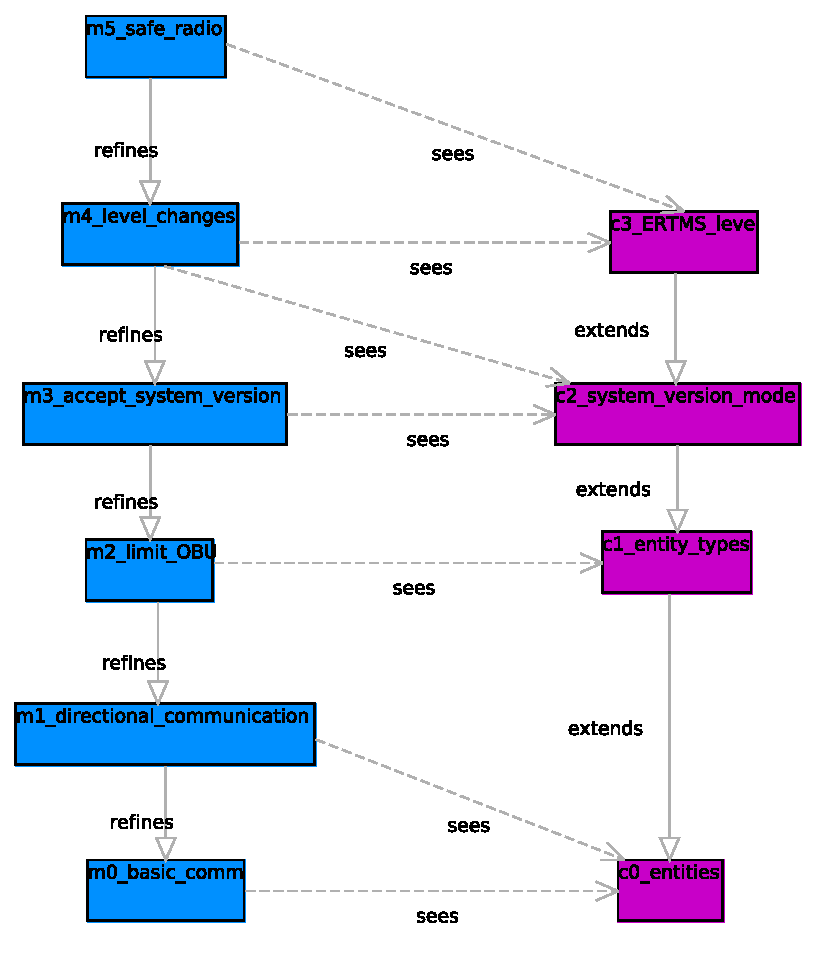
\includegraphics[width=.65\textwidth]{Subset_026_comm_session}
  \caption{Overview on State Machine and Context Hierarchy}
  \label{fig:model-overview}
\end{figure}

The modeling starts with the very abstract possibility to establish and to
terminate a communication session in the machine $m0$, the set of entities is
defined in the context $c0$. This basic functionality is refined in the
succeeding machines to incorporate the different stages of the protocol to
establish a session. The contexts further refine the entities to on-track and
on-board entities and limit the modeling to the point of view of an OBU.

The machine $m1$ discerns incoming and outgoing communication sessions, i.e.,
initiated by the modeled piece of equipment or by an external one. The context
$c1$ introduces the different types of equipment which are used in $m2$ to
refine the two different protocols for outgoing and incoming sessions and to
limit the model to the OBU point of view. $c2$ introduces the notion of
compatible systems. This is used in $m3$ to identify on-track equipment with a
compatible system version. This machine also discerns between accepting and
non-accepting RBCs to contact. $c3$ adds the different ERTMS levels and the
relevant train modes to the model. This is used in $m4$ to model the different
situations where a communication session must be established. $m5$ adds the
notion of safe radio connection as low-level prerequisite for a communication
session.

The representation of the state machines of the modeled protocols for
establishing a communication session is modeled implicitly. The model allows
sessions with different partners in parallel (but respects the constraints of
the specification like §3.5.3.5.2). The state of the protocol with different
partners is tracked by adding / removing these partners from sets representing
those different states of the protocol.

\section{Model Benefits}
\label{sec:model-highlights}

The Event-B model in Rodin has some interesting properties which are highlighted
here. Some stem from the fact that Rodin is well integrated into the Eclipse
platform which renders many useful plugins available, both those explicitly
developed for integration with Rodin, but also other without Rodin in mind.
Other interesting properties stem from the fact that Rodin and Event-B provide
an extensive proof support for properties.

\begin{itemize}
\item {\bf Refinement} The Event-B approach allows iterative development based
  on refinement. This allows starting modeling with a very abstract machine and
  then step-wise adding more detailed behavior. Rodin generates all the
  necessary proof obligations which are required to assure correct refinement.
\item {\bf Requirements Tracing} Rodin provides an extensible EMF model,
  therefore it is easily possible to trace requirements using the requirements
  modeling framework of Eclipse (RMF) via the ProR plugin. This allows the usage
  of requirement documents in the OMG standardized Requirements Interchange
  Format (ReqIF).
\item {\bf Model Animation} The Event-B model can be animated via different
  plugins, e.g., ProB or AnimB. This allows the simulation of the model, by
  clicking on the activated events and tracking the resulting state of the
  variables. This technique allows to examine the run-time behavior of the
  model, e.g., for testing purposes. There is also ongoing development for a
  model-based testing plugin in Rodin, which will allow storing and replaying of
  event sequences.
\item {\bf Non-Testable Requirements} The Event-B model supports the
  specification of invariants which can be formally proven using the proof
  support of Rodin. This includes for example the non-testable requirement
  specified in the subset 076 for §3.5.3.2 (see
  Section~\ref{sec:machine-2-board}).
\item {\bf Safety Properties} Using Rodin's proof support and the formalization
  as invariants, it is possible to formalize and prove the identified safety
  property of the case study (see Section~\ref{sec:machine-3-accepting}).
\end{itemize}

\section{Detailed Model Description}
\label{sec:deta-model-descr}

This section describes in more detail the formal model, beginning from the most
abstract Event-B machine. For each refinement, in general only the important
changes will be shown, the complete model is available as a Rodin project. At
each step the additional modeled functionality and its representation will be
described.  In particular the initialization event is not shown for the refined
machines. If not mentioned explicitly, sets are initialized empty, integers with
value 0 and Boolean variables with false.


\subsection{Context 0 - Entities}
\label{sec:context-0-entities}

This context defines the type of entities with whom a communication session can
be established.  $my\_entity$ represents the piece of equipment which is
modeled.

% \documentclass[10pt,a4paper]{report}
% \usepackage[top=3cm, bottom=2.5cm, left=3cm, right=2.5cm] {geometry}
% \usepackage {bsymb,b2latex}
% \usepackage[utf8]{inputenc}
% \usepackage{fancyhdr,lastpage,color}
% \lhead{\rm An Event-B Specification of c0\_entities}
% \rhead {\rm Page \thepage~of \pageref{LastPage}}
% \lfoot{}\cfoot{}\rfoot{}
% \pagestyle{fancy}
% %---------------------------------------------------------
% \begin{document}
% \thispagestyle{empty}
\begin{description}
% \BTitle{c0\_entities}{22Jan2013}{01:58:17 PM}
\CONTEXT{c0\_entities}
\SETS
        \begin{description}
                \Item{ entities }
        \end{description}
\CONSTANTS
        \begin{description}
                \Item{ my\_entity }
        \end{description}
\AXIOMS
        \begin{description}
                \nItem{ axm1 }{ my\_entity \in  entities }	\end{description}
\END
\end{description}
% \end{document}


\subsection{Machine 0 - Basic Communication}
\label{sec:machine-0-basic}

This state machine represents the basic functionality. It allows for the
creation and the termination of a communication session with another entity. The
sessions are represented by the state variable ``session'' which can contain
values of type ``entities''. The respective events are triggered with a
parameter $l\_partner$ representing the communication partner.

\paragraph{Implemented Requirements}
\label{sec:impl-requ}

\begin{itemize}
\item each session allows for communication between two entities (cf. §3.5.2.1)
\end{itemize}

\begin{description}
\SEES{c0\_entities}
\VARIABLES
        \begin{description}
                \Item{ sessions }
        \end{description}
\INVARIANTS
        \begin{description}
                \nItem{ inv1 }{ sessions \subseteq  entities \setminus  \{ my\_entity\}  }
        \end{description}
\EVENTS
        \INITIALISATION\cmt{ }
                \begin{description}
                \BeginAct
                        \begin{description}
                        \nItem{ act1 }{ sessions :=  \emptyset  }
                        \end{description}
                \EndAct
                \end{description}
        \EVT {establish\_communication}
                \begin{description}
                \AnyPrm
                        \begin{description}
                        \ItemY{l\_partner }{ }
                        \end{description}
                \WhereGrd
                        \begin{description}
                        \nItemY{ grd1 }{ l\_partner \notin  sessions }{ }
                        \nItem{ grd2 }{ l\_partner \neq  my\_entity }
                        \end{description}
                \ThenAct
                        \begin{description}
                        \nItem{ act1 }{ sessions :=  sessions \bunion  \{ l\_partner\}  }
                        \end{description}
                \EndAct
                \end{description}
        \EVT {terminate\_communication}
                \begin{description}
                \AnyPrm
                        \begin{description}
                        \Item{l\_partner }
                        \end{description}
                \WhereGrd
                        \begin{description}
                        \nItem{ grd1 }{ l\_partner \in  sessions }
                        \end{description}
                \ThenAct
                        \begin{description}
                        \nItem{ act1 }{ sessions :=  sessions \setminus  \{ l\_partner\}  }
                        \end{description}
                \EndAct
                \end{description}
\END
\end{description}


\subsection{Machine 1 - Directional Communication}
\label{sec:mach-1-direct}

The first refinement of the machine refines the notion of communication session
to incoming sessions, i.e., where another entity initiates a session with
$my\_entity$ and outgoing sessions where $my\_entity$ initiates the session.

The data refinement is proven by the invariant which states that ``sessions'' is
equal to the disjoint union of ``outgoing\_sessions'' and
``incoming\_sessions''. The abstract ``establish\_session'' event is refined to
the two events ``incoming\_session'' and ``outgoing\_session''.

\thispagestyle{empty}
\begin{description}
\REFINES{m0\_basic\_comm}
\SEES{c0\_entities}
\VARIABLES
        \begin{description}
                \Item{ incoming\_sessions }
                \Item{ outgoing\_sessions }
        \end{description}
\INVARIANTS
        \begin{description}
                \nItemY{ inv1 }{ partition (sessions, incoming\_sessions, outgoing\_sessions) }{  }
        \end{description}
\EVENTS
        \EVT {incoming\_communication}
        \REF {establish\_communication}
                \begin{description}
                \AnyPrm
                        \begin{description}
                        \ItemY{l\_partner }{ }
                        \end{description}
                \WhereGrd
                        \begin{description}
                        \nItem{ grd1 }{ l\_partner \notin  incoming\_sessions \bunion  outgoing\_sessions }
                        \nItemY{ grd2 }{ l\_partner \neq  my\_entity }{ }
                        \end{description}
                \ThenAct
                        \begin{description}
                        \nItemY{ act1 }{ incoming\_sessions :=  incoming\_sessions \bunion  \{ l\_partner\}  }{  }
                        \end{description}
                \EndAct
                \end{description}
        \EVT {outgoing\_communciation}
        \REF {establish\_communication}
                \begin{description}
                \AnyPrm
                        \begin{description}
                        \ItemY{l\_partner }{ }
                        \end{description}
                \WhereGrd
                        \begin{description}
                        \nItem{ grd2 }{ l\_partner \neq  my\_entity }
                        \nItemY{ grd1 }{ l\_partner \notin  incoming\_sessions \bunion  outgoing\_sessions }{ }
                        \end{description}
                \ThenAct
                        \begin{description}
                        \nItem{ act1 }{ outgoing\_sessions :=  outgoing\_sessions \bunion  \{ l\_partner\}  }
                        \end{description}
                \EndAct
                \end{description}
        \EVT {terminate\_communication}
        \REF {terminate\_communication}
                \begin{description}
                \AnyPrm
                        \begin{description}
                        \Item{l\_partner }
                        \end{description}
                \WhereGrd
                        \begin{description}
                        \nItem{ grd1 }{ l\_partner \in  incoming\_sessions \bunion  outgoing\_sessions }
                        \end{description}
                \ThenAct
                        \begin{description}
                        \nItem{ act1 }{ incoming\_sessions :=  incoming\_sessions \setminus  \{ l\_partner\}  }
                        \nItem{ act2 }{ outgoing\_sessions :=  outgoing\_sessions \setminus  \{ l\_partner\}  }
                        \end{description}
                \EndAct
                \end{description}
\END
\end{description}


\subsection{Context 1 - Entity Types}
\label{sec:context-1-entity}

The first context extension introduces the different types of entities relevant
in this requirement subset, i.e., on-board unit (OBU), radio in-fill unit (RIU)
or radio block centre (RBC). Every entity has a unique type. The goal is to
model the communication protocol from the point of view of an OBU, therefore the
type of $my\_entity$ is restricted to OBU.

\documentclass[10pt,a4paper]{report}
\usepackage[top=3cm, bottom=2.5cm, left=3cm, right=2.5cm] {geometry}
\usepackage {bsymb,b2latex}
\usepackage[utf8]{inputenc}
\usepackage{fancyhdr,lastpage,color}
\lhead{\rm An Event-B Specification of c1\_entity\_types}
\rhead {\rm Page \thepage~of \pageref{LastPage}}
\lfoot{}\cfoot{}\rfoot{}
\pagestyle{fancy}
%---------------------------------------------------------
\begin{document}
\thispagestyle{empty}
\begin{description}
\BTitle{c1\_entity\_types}{22Jan2013}{01:58:17 PM}
\CONTEXT{c1\_entity\_types}
\EXTENDS{c0\_entities}
\CONSTANTS
	\begin{description}
		\Item{ RBC }
		\Item{ RIU }
		\ItemY{ OBU }{}
		\Item{ on\_track }
		\ItemY{ on\_board }{}
	\end{description}
\AXIOMS
	\begin{description}
		\nItem{ axm1 }{ partition(entities,RBC,RIU,OBU) }\cmt{ }
		\nItem{ axm2 }{ on\_track = RIU \bunion  RBC }		\nItem{ axm3 }{ on\_board = OBU }\cmt{ }
		\nItem{ axm4 }{ my\_entity \in  on\_board }	\end{description}
\END
\end{description}
\end{document}


\subsection{Machine 2 - On Board Modeling}
\label{sec:machine-2-board}

The next machine refinement adds the notion of being contacted by an on-track
entity to establish a communication session. It also adds the first state of the
protocol, i.e., entities which should be contacted with the ``Initiation of a
communication session'' message. On-track entities which order ``my\_entity'' to
contact are stored in the ``contacted\_by'' set, entities to which the first
message is sent by ``my\_entity'' are stored in the set ``contacted',
representing those which are in the first stage of the protocol.

The invariants prove that $my\_entity$ will only be in contact with on-track
entities and that any entities which are considered for a communication session
are on-track entities. Any entity with whom there is already a communication
session will not be considered for another session, and finally no radio in-fill
unit can initiate a communication session with $my\_entity$.

\paragraph{Implemented Requirements}
\label{sec:impl-requ-1}

\begin{itemize}
\item It shall be possible for OBU and RBC to initiate communication session
  (cf. §3.5.3.1)
\item RIU cannot initiate a communication session (cf. §3.5.3.2)

This invariant is marked as non-testable in Subset-076.
\end{itemize}

The other invariants ensure that a communication partner is not in different
states of the communication protocol at the same time. A session protocol can be
started by the order to contact an RBC or directly by the OBU.

\documentclass[10pt,a4paper]{report}
\usepackage[top=3cm, bottom=2.5cm, left=3cm, right=2.5cm] {geometry}
\usepackage {bsymb,b2latex}
\usepackage[utf8]{inputenc}
\usepackage{fancyhdr,lastpage,color}
\lhead{\rm An Event-B Specification of m2\_limit\_OBU}
\rhead {\rm Page \thepage~of \pageref{LastPage}}
\lfoot{}\cfoot{}\rfoot{}
\pagestyle{fancy}
%---------------------------------------------------------
\begin{document}
\thispagestyle{empty}
\begin{description}
\BTitle{m2\_limit\_OBU}{22Jan2013}{01:58:17 PM}
\MACHINE{m2\_limit\_OBU}
\REFINES{m1\_directional\_communication}
\SEES{c1\_entity\_types}
\VARIABLES
	\begin{description}
		\Item{ incoming\_sessions }
		\ItemY{ outgoing\_sessions }{}
		\Item{ contacted }
		\ItemY{ contacted\_by }{}
	\end{description}
\INVARIANTS
	\begin{description}
		\nItemY{ inv1 }{ incoming\_sessions \bunion  outgoing\_sessions \subseteq  on\_track }{ 		\\\hspace*{1,4 cm}  limit model to OBU -$>$  only on$\_$track communication partners }
		\nItemY{ inv2 }{ contacted \subseteq  on\_track }{  }
		\nItemY{ inv3 }{ contacted\_by \subseteq  on\_track }{  }
		\nItem{ inv4 }{ contacted\_by \binter  (incoming\_sessions \bunion  outgoing\_sessions) = \emptyset  }
		\nItemY{ inv5 }{ contacted \binter  (incoming\_sessions \bunion  outgoing\_sessions) = \emptyset  }{  }
		\nItem{ inv6 }{ incoming\_sessions \binter  RIU = \emptyset  }
	\end{description}
\EVENTS
	\INITIALISATION
		\\\textit{extended}\cmt{ }
		\begin{description}
		\BeginAct
			\begin{description}
			\nItemX{ act2 }{ incoming\_sessions :=  \emptyset  }
			\nItemX{ act3 }{ outgoing\_sessions :=  \emptyset  }
			\nItem{ act4 }{ contacted :=  \emptyset  }
			\nItem{ act5 }{ contacted\_by :=  \emptyset  }
			\end{description}
		\EndAct
		\end{description}
	\EVT {incoming\_communication}
	\EXTD {incoming\_communication}
		\begin{description}
		\AnyPrm
			\begin{description}
			\ItemXY{l\_partner }{ }
			\end{description}
		\WhereGrd
			\begin{description}
			\nItemX{ grd1 }{ l\_partner \notin  incoming\_sessions \bunion  outgoing\_sessions }
			\nItemXY{ grd2 }{ l\_partner \in  entities \setminus  \{ l\_partner\}  }{ } 
			\nItem{ grd3 }{ l\_partner \in  on\_track \setminus  RIU }
			\end{description}
		\ThenAct
			\begin{description}
			\nItemXY{ act1 }{ incoming\_sessions :=  incoming\_sessions \bunion  \{ l\_partner\}  }{  }
			\end{description}
		\EndAct
		\end{description}
	\EVT {outgoing\_communciation}
	\EXTD {outgoing\_communciation}
		\begin{description}
		\AnyPrm
			\begin{description}
			\ItemXY{l\_partner }{ }
			\end{description}
		\WhereGrd
			\begin{description}
			\nItemX{ grd2 }{ l\_partner \in  entities \setminus  \{ l\_partner\}  }
			\nItemXY{ grd1 }{ l\_partner \notin  incoming\_sessions \bunion  outgoing\_sessions }{ } 
			\nItem{ grd3 }{ l\_partner \in  on\_track }
			\end{description}
		\ThenAct
			\begin{description}
			\nItemX{ act1 }{ outgoing\_sessions :=  outgoing\_sessions \bunion  \{ l\_partner\}  }
			\end{description}
		\EndAct
		\end{description}
	\EVT {receive\_contact\_order}\cmt{		\\\hspace*{4,8 cm}  RBC can order contact (cf. 3.5.3.4.b) }
		\begin{description}
		\AnyPrm
			\begin{description}
			\Item{l\_partner }
			\end{description}
		\WhereGrd
			\begin{description}
			\nItemY{ grd1 }{ l\_partner \notin  contacted \bunion  contacted\_by \bunion  incoming\_sessions \bunion  outgoing\_sessions }{ } 
			\nItem{ grd2 }{ l\_partner \in  on\_track }
			\end{description}
		\ThenAct
			\begin{description}
			\nItem{ act1 }{ contacted\_by :=  contacted\_by \bunion  \{ l\_partner\}  }
			\end{description}
		\EndAct
		\end{description}
	\EVT {initiate\_session\_after\_contact}\cmt{		\\\hspace*{6,6 cm}  (cf. 3.5.3.4 b) / (cf. 3.5.3.5.2) }
		\begin{description}
		\AnyPrm
			\begin{description}
			\Item{l\_partner }
			\end{description}
		\WhereGrd
			\begin{description}
			\nItem{ grd1 }{ l\_partner \notin  incoming\_sessions \bunion  outgoing\_sessions \bunion  contacted }
			\nItemY{ grd2 }{ l\_partner \in  contacted\_by }{ } 
			\end{description}
		\ThenAct
			\begin{description}
			\nItemY{ act1 }{ contacted :=  contacted \bunion  \{ l\_partner\}  }{  }
			\nItemY{ act2 }{ contacted\_by :=  contacted\_by \setminus  \{ l\_partner\}  }{  }
			\end{description}
		\EndAct
		\end{description}
	\EVT {initiate\_session\_no\_contact}\cmt{		\\\hspace*{6 cm}  no contact order, i.e., one ofthe other cases of 3.5.3.4 }
		\begin{description}
		\AnyPrm
			\begin{description}
			\ItemY{l\_partner }{ }
			\end{description}
		\WhereGrd
			\begin{description}
			\nItem{ grd5 }{ l\_partner \notin  incoming\_sessions \bunion  outgoing\_sessions \bunion  contacted \bunion  contacted\_by }
			\nItemY{ grd3 }{ l\_partner \in  on\_track }{ } 
			\end{description}
		\ThenAct
			\begin{description}
			\nItemY{ act2 }{ contacted :=  contacted \bunion  \{ l\_partner\}  }{  }
			\end{description}
		\EndAct
		\end{description}
	\EVT {terminate\_communication}
	\EXTD {terminate\_communication}
		\begin{description}
		\AnyPrm
			\begin{description}
			\ItemX{l\_partner }
			\end{description}
		\WhereGrd
			\begin{description}
			\nItemX{ grd1 }{ l\_partner \in  incoming\_sessions \bunion  outgoing\_sessions }
			\end{description}
		\ThenAct
			\begin{description}
			\nItemX{ act1 }{ incoming\_sessions :=  incoming\_sessions \setminus  \{ l\_partner\}  }
			\nItemX{ act2 }{ outgoing\_sessions :=  outgoing\_sessions \setminus  \{ l\_partner\}  }
			\end{description}
		\EndAct
		\end{description}
\END
\end{description}
\end{document}


\subsection{Context 2 - System Version Compatibility}
\label{sec:context-2-system}

The next context extension introduces the notion of compatible system
versions. This is modeled as a static property of the on-track equipment
wrt. $my\_entity$, i.e., the context axiom that ``system\_version\_compatible''
is a subset of all on-track entities. On this level of abstraction, there is no
need for a finer grained notion of compatibility.

% \documentclass[10pt,a4paper]{report}
% \usepackage[top=3cm, bottom=2.5cm, left=3cm, right=2.5cm] {geometry}
% \usepackage {bsymb,b2latex}
% \usepackage[utf8]{inputenc}
% \usepackage{fancyhdr,lastpage,color}
% \lhead{\rm An Event-B Specification of c2\_system\_version\_mode}
% \rhead {\rm Page \thepage~of \pageref{LastPage}}
% \lfoot{}\cfoot{}\rfoot{}
% \pagestyle{fancy}
% %---------------------------------------------------------
% \begin{document}
% \thispagestyle{empty}
\begin{description}
\EXTENDS{c1\_entity\_types}
\CONSTANTS
        \begin{description}
                \Item{ system\_version\_compatible }
        \end{description}
\AXIOMS
        \begin{description}
                \nItem{ axm1 }{ system\_version\_compatible \subseteq  on\_track }	\end{description}
\END
\end{description}


\subsection{Machine 3 - Accepting RBC and System Version}
\label{sec:machine-3-accepting}

The next machine refines the contact order events by discerning between the
orders to contact an accepting or a non-accepting RBC. The notion of being an
accepting RBC is considered to be a dynamic property and therefore modeled as a
variable, i.e., the set ``accepting''.

The ``receive\_contact\_order'' event is refined by two separate events, one for
orders for an accepting RBC and one for a non-accepting RBC. The
``outgoing\_communication'' event is refined by two events, one for a compatible
system version and the other for an incompatible one.

Furthermore, a just established communication session with on-track equipment
with an incompatible system version will be terminated immediately after
receiving this information. This is modeled by the set ``terminating\_session''
which holds values of type entities. Only those communication sessions in this
set can be closed by the termination event.

\paragraph{Implemented Requirements}
\label{sec:impl-requ-2}

\begin{itemize}
\item In case of a non-accepting RBC, all existing communication sessions with
  other RBCs must be terminated (cf. §3.5.3.5.2)
\item After the system version  is received by the OBU, the communication
  session is considered established and (cf. §3.5.3.8)
  \begin{itemize}
  \item if the system version is compatible, the OBU shall send the session
    established message to track-side (cf. 3.5.3.8.a)
  \item if the system version is incompatible, the OBU shall terminate the
    session (cf. 3.5.3.8.b)
  \end{itemize}
\item Any RBC which is contacted and with whom a communication session is
  established has a compatible system version (safety requirement from
  requirements document).
\end{itemize}

\begin{description}
\REFINES{m2\_limit\_OBU}
\SEES{c2\_system\_version\_mode}
\VARIABLES
        \begin{description}
                \ItemY{ terminating\_sessions }{}
                \Item{ accepting }
        \end{description}
\INVARIANTS
        \begin{description}
                \nItemY{ inv2 }{ RBC \binter  outgoing\_sessions \setminus  terminating\_sessions \subseteq  system\_version\_compatible }{           }
                \nItemY{ inv3 }{ accepting \subseteq  RBC }{}
                \nItemY{ inv4 }{ terminating\_sessions \subseteq  on\_track }{  }
        \end{description}
\EVENTS
        \EVT {receive\_information\_compatible}
        \EXTD {outgoing\_communciation}
                \begin{description}
                \AnyPrm
                        \begin{description}
                        \ItemXY{l\_partner }{ }
                        \end{description}
                \WhereGrd
                        \begin{description}
                        \nItemXY{ grd3 }{ l\_partner \in  contacted }{ }
                        \nItem{ grd4 }{ l\_partner \in  system\_version\_compatible }
                        \end{description}
                \ThenAct
                        \begin{description}
                        \nItemX{ act1 }{ outgoing\_sessions :=  outgoing\_sessions \bunion  \{ l\_partner\}  }
                        \nItemX{ act2 }{ contacted :=  contacted \setminus  \{ l\_partner\}  }
                        \end{description}
                \EndAct
                \end{description}
        \EVT {receive\_information\_incompatible}
        \EXTD {outgoing\_communciation}
                \begin{description}
                \AnyPrm
                        \begin{description}
                        \ItemXY{l\_partner }{ }
                        \end{description}
                \WhereGrd
                        \begin{description}
                        \nItemXY{ grd3 }{ l\_partner \in  contacted }{ }
                        \nItem{ grd4 }{ l\_partner \notin  system\_version\_compatible }
                        \end{description}
                \ThenAct
                        \begin{description}
                        \nItemX{ act1 }{ outgoing\_sessions :=  outgoing\_sessions \bunion  \{ l\_partner\}  }
                        \nItemX{ act2 }{ contacted :=  contacted \setminus  \{ l\_partner\}  }
                        \nItem{ act3 }{ terminating\_sessions :=  terminating\_sessions \bunion  \{ l\_partner\}  }
                        \end{description}
                \EndAct
                \end{description}
        \EVT {receive\_contact\_order\_accept}\cmt{}
        \REF {receive\_contact\_order}
                \begin{description}
                \AnyPrm
                        \begin{description}
                        \Item{l\_partner }
                        \end{description}
                \WhereGrd
                        \begin{description}
                        \nItemY{ grd1 }{ l\_partner \notin  contacted \bunion  contacted\_by \bunion  incoming\_sessions \bunion  outgoing\_sessions }{ }
                        \nItemY{ grd3 }{ l\_partner \in  RIU \bunion  (RBC \binter  accepting) }{ }
                        \end{description}
                \ThenAct
                        \begin{description}
                        \nItem{ act1 }{ contacted\_by :=  contacted\_by \bunion  \{ l\_partner\}  }
                        \end{description}
                \EndAct
                \end{description}
        \EVT {receive\_contact\_order\_non\_accept}\cmt{}
        \REF {receive\_contact\_order}
                \begin{description}
                \AnyPrm
                        \begin{description}
                        \Item{l\_partner }
                        \end{description}
                \WhereGrd
                        \begin{description}
                        \nItemY{ grd1 }{ l\_partner \notin  contacted \bunion  contacted\_by \bunion  incoming\_sessions \bunion  outgoing\_sessions }{ }
                        \nItem{ grd3 }{ l\_partner \in  RIU \bunion  (RBC \setminus  accepting) }
                        \end{description}
                \ThenAct
                        \begin{description}
                        \nItem{ act1 }{ contacted\_by :=  contacted\_by \bunion  \{ l\_partner\}  }
                        \nItem{ act2 }{ terminating\_sessions :=  terminating\_sessions \bunion  (RBC \binter  (incoming\_sessions \bunion  outgoing\_sessions)) }
                        \end{description}
                \EndAct
                \end{description}
        \EVT {terminate\_communication}
        \EXTD {terminate\_communication}
                \begin{description}
                \AnyPrm
                        \begin{description}
                        \ItemX{l\_partner }
                        \end{description}
                \WhereGrd
                        \begin{description}
                        \nItemX{ grd1 }{ l\_partner \in  incoming\_sessions \bunion  outgoing\_sessions }
                        \nItem{ grd2 }{ l\_partner \in  terminating\_sessions }
                        \end{description}
                \ThenAct
                        \begin{description}
                        \nItemX{ act1 }{ incoming\_sessions :=  incoming\_sessions \setminus  \{ l\_partner\}  }
                        \nItemX{ act2 }{ outgoing\_sessions :=  outgoing\_sessions \setminus  \{ l\_partner\}  }
                        \nItem{ act3 }{ terminating\_sessions :=  terminating\_sessions \setminus  \{ l\_partner\}  }
                        \end{description}
                \EndAct
                \end{description}
        \EVT {make\_RBC\_accepting}
                \begin{description}
                \AnyPrm
                        \begin{description}
                        \ItemY{l\_partner }{ }
                        \end{description}
                \WhereGrd
                        \begin{description}
                        \nItem{ grd1 }{ l\_partner \in  RBC }
                        \end{description}
                \ThenAct
                        \begin{description}
                        \nItem{ act1 }{ accepting :=  accepting \bunion  \{ l\_partner\}  }
                        \end{description}
                \EndAct
                \end{description}
        \EVT {make\_RBC\_non\_accepting}
                \begin{description}
                \AnyPrm
                        \begin{description}
                        \Item{l\_partner }
                        \end{description}
                \WhereGrd
                        \begin{description}
                        \nItem{ grd1 }{ l\_partner \in  accepting }
                        \end{description}
                \ThenAct
                        \begin{description}
                        \nItem{ act1 }{ accepting :=  accepting \setminus  \{ l\_partner\}  }
                        \end{description}
                \EndAct
                \end{description}
\END
\end{description}


\subsection{Context 3 - ERTMS Levels}
\label{sec:context-3-ertms}

The third context introduces the notion of the different ERTMS and the notion of
the mission status of a train. The modeled statuses are start of mission (SOM),
end of mission (EOM) and the abstract notion of within a mission (MIS), i.e.,
anything between start and end of the current train mission. At this level of
refinement, a more detailed modeling is not necessary.

\begin{description}
\CONTEXT{c3\_ERTMS\_level}
\SETS
        \begin{description}
                \ItemY{ ERTMS\_level }{ }
                \Item{ train\_status }
        \end{description}
\CONSTANTS
        \begin{description}
                \ItemY{ NTC }{}
                \Item{ L0 }
                \Item{ L1 }
                \Item{ L2 }
                \ItemY{ L3 }{}
                \ItemY{ SOM }{start of mission}
                \ItemY{ EOM }{end of mission}
                \ItemY{ MIS }{while mission}
        \end{description}
\AXIOMS
        \begin{description}
                \nItem{ axm1 }{ partition(ERTMS\_level, \{ NTC, L0, L1, L2, L3\} ) }		\nItem{ axm2 }{ partition(train\_status, \{ SOM, EOM, MIS\} ) }	\end{description}
\END
\end{description}



\subsection{Machine 4 - ERTMS Level Changes}
\label{sec:machine-4-ertms}

The next refined machine implements the different causes which can trigger the
establishing of a communication session. The corresponding events refine the
abstract ``initiate\_session\_no\_contact'' event. For this, the current ERTMS
level of the train is tracked, as well as its current mission status.

The indication of a level change, a mission status change, a manual level change
and an announced radio hole is modeled by events. These events modify the
corresponding indicator variables to signal a change and they modify the
corresponding state variables.

This can be illustrated using the manual level change event as example: the
Boolean variable ``signal\_manual\_level\_change'' indicates that the driver
manually changed the ERTMS level. It is changed by the ``manual\_change\_level''
event which is parametrized with the new level and which also modifies the
``current\_level'' variable which models the current ERTMS level. If the new
level is 2 or 3, then the train is required to establish a communication session
with trackside. This is realized in the
``initiate\_session\_no\_contact\_manual\_change'' event which reset the
indication variable once the entity has been contacted.  Similar events model
the initiation because of non-manual level change, mission status change and
announced radio holes.

\paragraph{Implemented Requirements}
\label{sec:impl-requ-3}

\begin{itemize}
\item The on-board shall establish a communication session (cf. §3.5.3.4)
  \begin{itemize}
  \item at start of mission (only if level 2 or 3) (cf. §3.5.3.4.a)
  \item if ordered from trackside (cf. §3.5.3.4.b)
  \item If a mode change, not considered as an End of Mission, has to be
    reported to the RBC (only if level 2 or 3) (cf. §3.5.3.4.c)
  \item If the driver has manually changed the level to 2 or 3 (cf. §3.5.3.4.d)
  \item When the train front reaches the end of an announced radio hole
    (cf. §3.5.3.4.e)
  \end{itemize}
\end{itemize}

\begin{description}
\REFINES{m3\_accept\_system\_version}
\SEES{c3\_ERTMS\_level}
\VARIABLES
        \begin{description}
                \ItemY{ current\_level }{}
                \ItemY{ signal\_level\_change }{}
                \ItemY{ current\_status }{}
                \ItemY{ signal\_status\_change }{}
                \ItemY{ signal\_manual\_level\_change }{}
                \ItemY{ position\_radio\_hole }{}
                \Item{ signal\_radio\_hole }
        \end{description}
\INVARIANTS
        \begin{description}
                \nItemY{ inv1 }{ current\_level \in  ERTMS\_level }{  }
                \nItemY{ inv2 }{ signal\_level\_change \in  BOOL }{  }
                \nItem{ inv3 }{ current\_status \in  train\_status }
                \nItemY{ inv4 }{ signal\_status\_change \in  BOOL }{  }
                \nItemY{ inv5 }{ signal\_manual\_level\_change \in  BOOL }{  }
                \nItemY{ inv6 }{ position\_radio\_hole \in  BOOL }{  }
                \nItem{ inv7 }{ signal\_radio\_hole \in  BOOL }
        \end{description}
\EVENTS
        \EVT {manual\_change\_level}
                \begin{description}
                \AnyPrm
                        \begin{description}
                        \ItemY{l\_level }{ }
                        \end{description}
                \WhereGrd
                        \begin{description}
                        \nItemY{ grd1 }{ l\_level \in  ERTMS\_level }{ }
                        \nItem{ grd2 }{ signal\_manual\_level\_change = FALSE }
                        \nItem{ grd3 }{ signal\_level\_change = FALSE }
                        \end{description}
                \ThenAct
                        \begin{description}
                        \nItemY{ act1 }{ signal\_manual\_level\_change :=  TRUE }{  }
                        \nItem{ act2 }{ current\_level :=  l\_level }
                        \end{description}
                \EndAct
                \end{description}
        \EVT {change\_level}
                \begin{description}
                \AnyPrm
                        \begin{description}
                        \ItemY{l\_level }{ }
                        \end{description}
                \WhereGrd
                        \begin{description}
                        \nItemY{ grd1 }{ l\_level \in  ERTMS\_level }{ }
                        \nItemY{ grd2 }{ signal\_manual\_level\_change = FALSE }{ }
                        \nItem{ grd3 }{ signal\_level\_change = FALSE }
                        \end{description}
                \ThenAct
                        \begin{description}
                        \nItemY{ act1 }{ current\_level :=  l\_level }{  }
                        \nItem{ act2 }{ signal\_level\_change :=  TRUE }
                        \end{description}
                \EndAct
                \end{description}
        \EVT {initiate\_session\_no\_contact\_accept}
        \EXTD {initiate\_session\_no\_contact\_accept}
                \begin{description}
                \AnyPrm
                        \begin{description}
                        \ItemXY{l\_partner }{ }
                        \end{description}
                \WhereGrd
                        \begin{description}
                        \nItemX{ grd5 }{ l\_partner \notin  incoming\_sessions \bunion  outgoing\_sessions \bunion  contacted \bunion  contacted\_by }
                        \nItemXY{ grd3 }{ l\_partner \in  RIU \bunion  (RBC \binter  accepting) }{ }
                        \end{description}
                \ThenAct
                        \begin{description}
                        \nItemXY{ act2 }{ contacted :=  contacted \bunion  \{ l\_partner\}  }{  }
                        \end{description}
                \EndAct
                \end{description}
        \EVT {initiate\_session\_no\_contact\_non\_accept}
        \EXTD {initiate\_session\_no\_contact\_non\_accept}
                \begin{description}
                \AnyPrm
                        \begin{description}
                        \ItemXY{l\_partner }{ }
                        \end{description}
                \WhereGrd
                        \begin{description}
                        \nItemX{ grd5 }{ l\_partner \notin  incoming\_sessions \bunion  outgoing\_sessions \bunion  contacted \bunion  contacted\_by }
                        \nItemXY{ grd3 }{ l\_partner \in  RIU \bunion  (RBC \setminus  accepting) }{ }
                        \end{description}
                \ThenAct
                        \begin{description}
                        \nItemXY{ act2 }{ contacted :=  contacted \bunion  \{ l\_partner\}  }{  }
                        \nItemX{ act3 }{ terminating\_sessions :=  terminating\_sessions \bunion  (RBC \binter  (incoming\_sessions \bunion  outgoing\_sessions)) }
                        \end{description}
                \EndAct
                \end{description}
        \EVT {initiate\_session\_no\_contact\_manual\_change\_accept}
        \EXTD {initiate\_session\_no\_contact\_accept}
                \begin{description}
                \AnyPrm
                        \begin{description}
                        \ItemXY{l\_partner }{ }
                        \end{description}
                \WhereGrd
                        \begin{description}
                        \nItemX{ grd5 }{ l\_partner \notin  incoming\_sessions \bunion  outgoing\_sessions \bunion  contacted \bunion  contacted\_by }
                        \nItemXY{ grd3 }{ l\_partner \in  RIU \bunion  (RBC \binter  accepting) }{ }
                        \nItem{ grd6 }{ current\_level \in  \{ L2, L3\}  }
                        \nItem{ grd7 }{ signal\_manual\_level\_change = TRUE }
                        \end{description}
                \ThenAct
                        \begin{description}
                        \nItemXY{ act2 }{ contacted :=  contacted \bunion  \{ l\_partner\}  }{  }
                        \nItem{ act3 }{ signal\_manual\_level\_change :=  FALSE }
                        \end{description}
                \EndAct
                \end{description}
        \EVT {initiate\_session\_no\_contact\_manual\_change\_non\_accept}
        \REF {initiate\_session\_no\_contact\_non\_accept}
                \begin{description}
                \AnyPrm
                        \begin{description}
                        \ItemY{l\_partner }{ }
                        \end{description}
                \WhereGrd
                        \begin{description}
                        \nItem{ grd5 }{ l\_partner \notin  incoming\_sessions \bunion  outgoing\_sessions \bunion  contacted \bunion  contacted\_by }
                        \nItemY{ grd3 }{ l\_partner \in  RIU \bunion  (RBC \setminus  accepting) }{ }
                        \nItem{ grd6 }{ current\_level \in  \{ L2, L3\}  }
                        \nItem{ grd7 }{ signal\_manual\_level\_change = TRUE }
                        \end{description}
                \ThenAct
                        \begin{description}
                        \nItemY{ act2 }{ contacted :=  contacted \bunion  \{ l\_partner\}  }{  }
                        \nItem{ act3 }{ terminating\_sessions :=  terminating\_sessions \bunion  (RBC \binter  (incoming\_sessions \bunion  outgoing\_sessions)) }
                        \end{description}
                \EndAct
                \end{description}
\END
\end{description}


\subsection{Machine 5 - Safe Radio Connection}
\label{sec:machine-5-safe}

The next machine refinement specifies handling of the safe radio connection
which provides the necessary means to exchange protocol messages on a higher
level. The existing established safe radio connections are represented by the
set ``ER\_connections'' which holds values of type entities. Safe radio
connections which must be established are modeled by the set
``establish\_ER\_connections'' while ``terminated\_ER\_connections'' holds those
connections which timed-out. The indication variable ``signal\_RBC\_border''
signals the crossing of an RBC border which requires to establish a new safe
radio connection with a new RBC.

Establishing a communication session then works as follows: if one of the
conditions of §3.5.3.4 is fulfilled, the corresponding partner is added to the
set ``contacted''. This is a pre-condition of the events which open a safe radio
connection to a communication partner. The initiation message of the protocol is
considered to be sent when a communication partner is both ``contacted'' and
``ER\_connections'' set. The reception of the system version and the sending of
the system established message is modeled via the
``receive\_information\_compatible'' or ``receive\_information\_incompatible''
events. Established sessions with incompatible system versions are therefore in
the intersection of the ``sessions'' and ``terminating\_sessions'' sets.

\paragraph{Implemented Requirements}
\label{sec:impl-requ-4}

\begin{itemize}
\item Establish communication session after safe radio connection timeout
  (cf. §3.5.3.4.f)
\item If the communication session is established by an OBU, it shall be
  preformed according to the following steps (cf. §3.5.3.7)
  \begin{itemize}
  \item if part of ongoing start of mission procedure (cf. §3.5.3.7.a)
  \item if safe radio connection is set up (cf. §3.5.3.7.i)
  \item if end of mission is performed (cf. §3.5.3.7.iii)
  \item train passes level transition border (cf. §3.5.3.7.iv)
  \item order to establish connection with different non-accepting RBC
    (cf. §3.5.3.7.v)
  \item train passes RBC / RBC border (cf. §3.5.3.7.vi)
  \item train enters announced radio hole (cf. §3.5.3.7.vii)
  \item level 1 is left (RIU only) (cf. §3.5.3.7.viii)
  \end{itemize}
\end{itemize}

\begin{description}
\REFINES{m4\_level\_changes}
\SEES{c3\_ERTMS\_level}
\VARIABLES
        \begin{description}
                \ItemY{ ER\_connections }{}
                \ItemY{ terminated\_ER\_connections }{}
                \ItemY{ establish\_ER\_connection }{}
                \Item{ signal\_RBC\_border }{}
        \end{description}
\INVARIANTS
        \begin{description}
                \nItemY{ inv1 }{ terminated\_ER\_connections \subseteq  on\_track }{  }
                \nItemY{ inv2 }{ establish\_ER\_connection \subseteq  on\_track }{  }
                \nItemY{ inv3 }{ (incoming\_sessions \bunion  outgoing\_sessions) \subseteq  ER\_connections }{  }
                \nItem{ inv4 }{ signal\_RBC\_border \in  BOOL }
        \end{description}
\EVENTS
        \EVT {incoming\_communication}
        \EXTD {incoming\_communication}
                \begin{description}
                \AnyPrm
                        \begin{description}
                        \ItemXY{l\_partner }{ }
                        \end{description}
                \WhereGrd
                        \begin{description}
                        \nItemX{ grd1 }{ l\_partner \notin  incoming\_sessions \bunion  outgoing\_sessions }
                        \nItemXY{ grd3 }{ l\_partner \in  on\_track \setminus  RIU }{ }
                        \nItemXY{ grd4 }{ l\_partner \notin  contacted }{ }
                        \nItemX{ grd5 }{ l\_partner \notin  contacted\_by }
                        \nItem{ grd6 }{ l\_partner \in  ER\_connections }
                        \end{description}
                \ThenAct
                        \begin{description}
                        \nItemXY{ act1 }{ incoming\_sessions :=  incoming\_sessions \bunion  \{ l\_partner\}  }{  }
                        \end{description}
                \EndAct
                \end{description}
        \EVT {receive\_information\_compatible}
        \EXTD {receive\_information\_compatible}
                \begin{description}
                \AnyPrm
                        \begin{description}
                        \ItemXY{l\_partner }{ }
                        \end{description}
                \WhereGrd
                        \begin{description}
                        \nItemXY{ grd3 }{ l\_partner \in  contacted }{ }
                        \nItemX{ grd4 }{ l\_partner \in  system\_version\_compatible }
                        \nItem{ grd5 }{ l\_partner \in  ER\_connections }
                        \end{description}
                \ThenAct
                        \begin{description}
                        \nItemX{ act1 }{ outgoing\_sessions :=  outgoing\_sessions \bunion  \{ l\_partner\}  }
                        \nItemX{ act2 }{ contacted :=  contacted \setminus  \{ l\_partner\}  }
                        \end{description}
                \EndAct
                \end{description}
        \EVT {receive\_information\_incompatible}
        \EXTD {receive\_information\_incompatible}
                \begin{description}
                \AnyPrm
                        \begin{description}
                        \ItemXY{l\_partner }{ }
                        \end{description}
                \WhereGrd
                        \begin{description}
                        \nItemXY{ grd3 }{ l\_partner \in  contacted }{ }
                        \nItemX{ grd4 }{ l\_partner \notin  system\_version\_compatible }
                        \nItem{ grd5 }{ l\_partner \in  ER\_connections }
                        \end{description}
                \ThenAct
                        \begin{description}
                        \nItemX{ act1 }{ outgoing\_sessions :=  outgoing\_sessions \bunion  \{ l\_partner\}  }
                        \nItemX{ act2 }{ contacted :=  contacted \setminus  \{ l\_partner\}  }
                        \nItemX{ act3 }{ terminating\_sessions :=  terminating\_sessions \bunion  \{ l\_partner\}  }
                        \end{description}
                \EndAct
                \end{description}
        \EVT {receive\_contact\_order\_accept}\cmt{		\\\hspace*{6,2 cm}  order to contact a RIU or accepting RBC }
        \EXTD {receive\_contact\_order\_accept}
                \begin{description}
                \AnyPrm
                        \begin{description}
                        \ItemX{l\_partner }
                        \end{description}
                \WhereGrd
                        \begin{description}
                        \nItemXY{ grd1 }{ l\_partner \notin  contacted \bunion  contacted\_by \bunion  incoming\_sessions \bunion  outgoing\_sessions }{ }
                        \nItemXY{ grd3 }{ l\_partner \in  RIU \bunion  (RBC \binter  accepting) }{}
                        \nItem{ grd4 }{ l\_partner \notin  terminated\_ER\_connections }
                        \end{description}
                \ThenAct
                        \begin{description}
                        \nItemX{ act1 }{ contacted\_by :=  contacted\_by \bunion  \{ l\_partner\}  }
                        \end{description}
                \EndAct
                \end{description}
        \EVT {receive\_contact\_order\_non\_accept}\cmt{}
        \EXTD {receive\_contact\_order\_non\_accept}
                \begin{description}
                \AnyPrm
                        \begin{description}
                        \ItemX{l\_partner }
                        \end{description}
                \WhereGrd
                        \begin{description}
                        \nItemXY{ grd1 }{ l\_partner \notin  contacted \bunion  contacted\_by \bunion  incoming\_sessions \bunion  outgoing\_sessions }{ }
                        \nItemX{ grd3 }{ l\_partner \in  RIU \bunion  (RBC \setminus  accepting) }
                        \nItem{ grd4 }{ l\_partner \notin  terminated\_ER\_connections }
                        \end{description}
                \ThenAct
                        \begin{description}
                        \nItemX{ act1 }{ contacted\_by :=  contacted\_by \bunion  \{ l\_partner\}  }
                        \nItemX{ act2 }{ terminating\_sessions :=  terminating\_sessions \bunion  (RBC \binter  (incoming\_sessions \bunion  outgoing\_sessions)) }
                        \end{description}
                \EndAct
                \end{description}
        \EVT {initiate\_session\_after\_contact\_accept}\cmt{		\\\hspace*{8 cm}  (cf. 3.5.3.4 b) / (cf. 3.5.3.5.2) }
        \EXTD {initiate\_session\_after\_contact}
                \begin{description}
                \AnyPrm
                        \begin{description}
                        \ItemX{l\_partner }
                        \end{description}
                \WhereGrd
                        \begin{description}
                        \nItemXY{ grd2 }{ l\_partner \in  contacted\_by }{ }
                        \nItemY{ grd3 }{ l\_partner \notin  terminated\_ER\_connections }{ }
                        \end{description}
                \ThenAct
                        \begin{description}
                        \nItemXY{ act1 }{ contacted :=  contacted \bunion  \{ l\_partner\}  }{  }
                        \nItemXY{ act2 }{ contacted\_by :=  contacted\_by \setminus  \{ l\_partner\}  }{  }
                        \nItem{ act3 }{ establish\_ER\_connection :=  establish\_ER\_connection \bunion  \{ l\_partner\}  }
                        \end{description}
                \EndAct
                \end{description}
        \EVT {initiate\_session\_no\_contact\_SOM\_accept}\cmt{		\\\hspace*{8,2 cm}  no contact order, i.e., one ofthe other cases of 3.5.3.4 }
        \EXTD {initiate\_session\_no\_contact\_SOM\_accept}
                \begin{description}
                \AnyPrm
                        \begin{description}
                        \ItemXY{l\_partner }{ }
                        \end{description}
                \WhereGrd
                        \begin{description}
                        \nItemX{ grd5 }{ l\_partner \notin  incoming\_sessions \bunion  outgoing\_sessions \bunion  contacted \bunion  contacted\_by }
                        \nItemXY{ grd3 }{ l\_partner \in  RIU \bunion  (RBC \binter  accepting) }{ }
                        \nItemXY{ grd6 }{ current\_status = SOM }{ }
                        \nItemX{ grd7 }{ current\_level \in  \{ L2, L3\}  }
                        \nItem{ grd8 }{ l\_partner \notin  terminated\_ER\_connections }
                        \end{description}
                \ThenAct
                        \begin{description}
                        \nItemXY{ act2 }{ contacted :=  contacted \bunion  \{ l\_partner\}  }{  }
                        \nItem{ act3 }{ establish\_ER\_connection :=  establish\_ER\_connection \bunion  \{ l\_partner\}  }
                        \end{description}
                \EndAct
                \end{description}
        \EVT {initiate\_session\_no\_contact\_SOM\_non\_accept}
        \EXTD {initiate\_session\_no\_contact\_SOM\_non\_accept}
                \begin{description}
                \AnyPrm
                        \begin{description}
                        \ItemXY{l\_partner }{ }
                        \end{description}
                \WhereGrd
                        \begin{description}
                        \nItemX{ grd5 }{ l\_partner \notin  incoming\_sessions \bunion  outgoing\_sessions \bunion  contacted \bunion  contacted\_by }
                        \nItemXY{ grd3 }{ l\_partner \in  RIU \bunion  (RBC \setminus  accepting) }{ }
                        \nItemX{ grd6 }{ current\_status = SOM }
                        \nItemX{ grd7 }{ current\_level \in  \{ L2, L3\}  }
                        \nItem{ grd8 }{ l\_partner \notin  terminated\_ER\_connections }
                        \end{description}
                \ThenAct
                        \begin{description}
                        \nItemXY{ act2 }{ contacted :=  contacted \bunion  \{ l\_partner\}  }{  }
                        \nItemX{ act3 }{ terminating\_sessions :=  terminating\_sessions \bunion  (RBC \binter  (incoming\_sessions \bunion  outgoing\_sessions)) }
                        \nItem{ act4 }{ establish\_ER\_connection :=  establish\_ER\_connection \bunion  \{ l\_partner\}  }
                        \end{description}
                \EndAct
                \end{description}
        \EVT {initiate\_session\_no\_contact\_mode\_change\_accept}
        \EXTD {initiate\_session\_no\_contact\_mode\_change\_accept}
                \begin{description}
                \AnyPrm
                        \begin{description}
                        \ItemXY{l\_partner }{ }
                        \end{description}
                \WhereGrd
                        \begin{description}
                        \nItemX{ grd5 }{ l\_partner \notin  incoming\_sessions \bunion  outgoing\_sessions \bunion  contacted \bunion  contacted\_by }
                        \nItemXY{ grd3 }{ l\_partner \in  RIU \bunion  (RBC \binter  accepting) }{ }
                        \nItemX{ grd6 }{ current\_level \in  \{ L2, L3\}  }
                        \nItemXY{ grd7 }{ signal\_mode\_change = TRUE }{ }
                        \nItemX{ grd8 }{ current\_status \neq  EOM }
                        \nItem{ grd9 }{ l\_partner \notin  terminated\_ER\_connections }
                        \end{description}
                \ThenAct
                        \begin{description}
                        \nItemXY{ act2 }{ contacted :=  contacted \bunion  \{ l\_partner\}  }{  }
                        \nItemX{ act3 }{ signal\_mode\_change :=  FALSE }
                        \nItem{ act4 }{ establish\_ER\_connection :=  establish\_ER\_connection \bunion  \{ l\_partner\}  }
                        \end{description}
                \EndAct
                \end{description}
        \EVT {initiate\_session\_no\_contact\_mode\_change\_non\_accept}
        \EXTD {initiate\_session\_no\_contact\_mode\_change\_non\_accept}
                \begin{description}
                \AnyPrm
                        \begin{description}
                        \ItemXY{l\_partner }{ }
                        \end{description}
                \WhereGrd
                        \begin{description}
                        \nItemX{ grd5 }{ l\_partner \notin  incoming\_sessions \bunion  outgoing\_sessions \bunion  contacted \bunion  contacted\_by }
                        \nItemXY{ grd3 }{ l\_partner \in  RIU \bunion  (RBC \setminus  accepting) }{ }
                        \nItemX{ grd6 }{ current\_level \in  \{ L2, L3\}  }
                        \nItemX{ grd7 }{ signal\_mode\_change = TRUE }
                        \nItemX{ grd8 }{ current\_status \neq  EOM }
                        \nItem{ grd9 }{ l\_partner \notin  terminated\_ER\_connections }
                        \end{description}
                \ThenAct
                        \begin{description}
                        \nItemXY{ act2 }{ contacted :=  contacted \bunion  \{ l\_partner\}  }{  }
                        \nItemX{ act3 }{ terminating\_sessions :=  terminating\_sessions \bunion  (RBC \binter  (incoming\_sessions \bunion  outgoing\_sessions)) }
                        \nItem{ act4 }{ establish\_ER\_connection :=  establish\_ER\_connection \bunion  \{ l\_partner\}  }
                        \end{description}
                \EndAct
                \end{description}
        \EVT {initiate\_session\_no\_contact\_manual\_change\_accept}
        \EXTD {initiate\_session\_no\_contact\_manual\_change\_accept}
                \begin{description}
                \AnyPrm
                        \begin{description}
                        \ItemXY{l\_partner }{ }
                        \end{description}
                \WhereGrd
                        \begin{description}
                        \nItemX{ grd5 }{ l\_partner \notin  incoming\_sessions \bunion  outgoing\_sessions \bunion  contacted \bunion  contacted\_by }
                        \nItemXY{ grd3 }{ l\_partner \in  RIU \bunion  (RBC \binter  accepting) }{ }
                        \nItemX{ grd6 }{ current\_level \in  \{ L2, L3\}  }
                        \nItemX{ grd7 }{ signal\_manual\_level\_change = TRUE }
                        \nItem{ grd8 }{ l\_partner \notin  terminated\_ER\_connections }
                        \end{description}
                \ThenAct
                        \begin{description}
                        \nItemXY{ act2 }{ contacted :=  contacted \bunion  \{ l\_partner\}  }{  }
                        \nItemX{ act3 }{ signal\_manual\_level\_change :=  FALSE }
                        \nItem{ act4 }{ establish\_ER\_connection :=  establish\_ER\_connection \bunion  \{ l\_partner\}  }
                        \end{description}
                \EndAct
                \end{description}
        \EVT {initiate\_session\_no\_contact\_manual\_change\_non\_accept}
        \EXTD {initiate\_session\_no\_contact\_manual\_change\_non\_accept}
                \begin{description}
                \AnyPrm
                        \begin{description}
                        \ItemXY{l\_partner }{ }
                        \end{description}
                \WhereGrd
                        \begin{description}
                        \nItemX{ grd5 }{ l\_partner \notin  incoming\_sessions \bunion  outgoing\_sessions \bunion  contacted \bunion  contacted\_by }
                        \nItemXY{ grd3 }{ l\_partner \in  RIU \bunion  (RBC \setminus  accepting) }{ }
                        \nItemX{ grd6 }{ current\_level \in  \{ L2, L3\}  }
                        \nItemX{ grd7 }{ signal\_manual\_level\_change = TRUE }
                        \nItem{ grd8 }{ l\_partner \notin  terminated\_ER\_connections }
                        \end{description}
                \ThenAct
                        \begin{description}
                        \nItemXY{ act2 }{ contacted :=  contacted \bunion  \{ l\_partner\}  }{  }
                        \nItemX{ act3 }{ terminating\_sessions :=  terminating\_sessions \bunion  (RBC \binter  (incoming\_sessions \bunion  outgoing\_sessions)) }
                        \nItem{ act4 }{ establish\_ER\_connection :=  establish\_ER\_connection \bunion  \{ l\_partner\}  }
                        \end{description}
                \EndAct
                \end{description}
        \EVT {initiate\_session\_no\_contact\_leave\_radio\_hole\_accept}
        \EXTD {initiate\_session\_no\_contact\_leave\_radio\_hole\_accept}
                \begin{description}
                \AnyPrm
                        \begin{description}
                        \ItemXY{l\_partner }{ }
                        \end{description}
                \WhereGrd
                        \begin{description}
                        \nItemX{ grd5 }{ l\_partner \notin  incoming\_sessions \bunion  outgoing\_sessions \bunion  contacted \bunion  contacted\_by }
                        \nItemXY{ grd3 }{ l\_partner \in  RIU \bunion  (RBC \binter  accepting) }{ }
                        \nItemX{ grd6 }{ position\_radio\_hole = FALSE }
                        \nItemX{ grd7 }{ signal\_radio\_hole = TRUE }
                        \nItem{ grd8 }{ l\_partner \notin  terminated\_ER\_connections }
                        \end{description}
                \ThenAct
                        \begin{description}
                        \nItemXY{ act2 }{ contacted :=  contacted \bunion  \{ l\_partner\}  }{  }
                        \nItemX{ act3 }{ signal\_radio\_hole :=  FALSE }
                        \nItem{ act4 }{ establish\_ER\_connection :=  establish\_ER\_connection \bunion  \{ l\_partner\}  }
                        \end{description}
                \EndAct
                \end{description}
        \EVT {initiate\_session\_no\_contact\_leave\_radio\_hole\_non\_accept}
        \EXTD {initiate\_session\_no\_contact\_leave\_radio\_hole\_non\_accept}
                \begin{description}
                \AnyPrm
                        \begin{description}
                        \ItemXY{l\_partner }{ }
                        \end{description}
                \WhereGrd
                        \begin{description}
                        \nItemX{ grd5 }{ l\_partner \notin  incoming\_sessions \bunion  outgoing\_sessions \bunion  contacted \bunion  contacted\_by }
                        \nItemXY{ grd3 }{ l\_partner \in  RIU \bunion  (RBC \setminus  accepting) }{ }
                        \nItemX{ grd6 }{ position\_radio\_hole = FALSE }
                        \nItemX{ grd7 }{ signal\_radio\_hole = TRUE }
                        \nItem{ grd8 }{ l\_partner \notin  terminated\_ER\_connections }
                        \end{description}
                \ThenAct
                        \begin{description}
                        \nItemXY{ act2 }{ contacted :=  contacted \bunion  \{ l\_partner\}  }{  }
                        \nItemX{ act3 }{ terminating\_sessions :=  terminating\_sessions \bunion  (RBC \binter  (incoming\_sessions \bunion  outgoing\_sessions)) }
                        \nItem{ act4 }{ establish\_ER\_connection :=  establish\_ER\_connection \bunion  \{ l\_partner\}  }
                        \end{description}
                \EndAct
                \end{description}
        \EVT {initiate\_session\_after\_timeout\_accept}
        \EXTD {initiate\_session\_no\_contact\_accept}
                \begin{description}
                \AnyPrm
                        \begin{description}
                        \ItemXY{l\_partner }{ }
                        \end{description}
                \WhereGrd
                        \begin{description}
                        \nItemX{ grd5 }{ l\_partner \notin  incoming\_sessions \bunion  outgoing\_sessions \bunion  contacted \bunion  contacted\_by }
                        \nItemXY{ grd3 }{ l\_partner \in  RIU \bunion  (RBC \binter  accepting) }{ }
                        \nItem{ grd6 }{ l\_partner \in  terminated\_ER\_connections }
                        \end{description}
                \ThenAct
                        \begin{description}
                        \nItemXY{ act2 }{ contacted :=  contacted \bunion  \{ l\_partner\}  }{  }
                        \nItem{ act3 }{ terminated\_ER\_connections :=  terminated\_ER\_connections \setminus  \{ l\_partner\}  }
                        \nItem{ act4 }{ establish\_ER\_connection :=  establish\_ER\_connection \bunion  \{ l\_partner\}  }
                        \end{description}
                \EndAct
                \end{description}
        \EVT {initiate\_session\_after\_timeout\_non\_accept}
        \EXTD {initiate\_session\_no\_contact\_non\_accept}
                \begin{description}
                \AnyPrm
                        \begin{description}
                        \ItemXY{l\_partner }{ }
                        \end{description}
                \WhereGrd
                        \begin{description}
                        \nItemX{ grd5 }{ l\_partner \notin  incoming\_sessions \bunion  outgoing\_sessions \bunion  contacted \bunion  contacted\_by }
                        \nItemXY{ grd3 }{ l\_partner \in  RIU \bunion  (RBC \setminus  accepting) }{ }
                        \nItem{ grd6 }{ l\_partner \in  terminated\_ER\_connections }
                        \end{description}
                \ThenAct
                        \begin{description}
                        \nItemXY{ act2 }{ contacted :=  contacted \bunion  \{ l\_partner\}  }{  }
                        \nItemX{ act3 }{ terminating\_sessions :=  terminating\_sessions \bunion  (RBC \binter  (incoming\_sessions \bunion  outgoing\_sessions)) }
                        \nItem{ act4 }{ terminated\_ER\_connections :=  terminated\_ER\_connections \setminus  \{ l\_partner\}  }
                        \nItem{ act5 }{ establish\_ER\_connection :=  establish\_ER\_connection \bunion  \{ l\_partner\}  }
                        \end{description}
                \EndAct
                \end{description}
        \EVT {establish\_ER\_connection\_SOM}
                \begin{description}
                \AnyPrm
                        \begin{description}
                        \Item{l\_partner }
                        \end{description}
                \WhereGrd
                        \begin{description}
                        \nItem{ grd1 }{ l\_partner \in  contacted }
                        \nItemY{ grd2 }{ l\_partner \in  establish\_ER\_connection }{ }
                        \nItem{ grd3 }{ current\_status = SOM }
                        \end{description}
                \ThenAct
                        \begin{description}
                        \nItem{ act1 }{ establish\_ER\_connection :=  establish\_ER\_connection \setminus  \{ l\_partner\}  }
                        \nItem{ act2 }{ ER\_connections :=  ER\_connections \bunion  \{ l\_partner\}  }
                        \end{description}
                \EndAct
                \end{description}
        \EVT {establish\_ER\_connection}
                \begin{description}
                \AnyPrm
                        \begin{description}
                        \ItemY{l\_partner }{ }
                        \end{description}
                \WhereGrd
                        \begin{description}
                        \nItem{ grd1 }{ l\_partner \in  contacted }
                        \nItem{ grd2 }{ l\_partner \in  establish\_ER\_connection }
                        \nItemY{ grd3 }{ current\_status \neq  SOM }{ }
                        \end{description}
                \ThenAct
                        \begin{description}
                        \nItem{ act1 }{ establish\_ER\_connection :=  establish\_ER\_connection \setminus  \{ l\_partner\}  }
                        \nItem{ act2 }{ ER\_connections :=  ER\_connections \bunion  \{ l\_partner\}  }
                        \end{description}
                \EndAct
                \end{description}
        \EVT {est\_perform\_end\_of\_mission}\cmt{}
                \begin{description}
                \AnyPrm
                        \begin{description}
                        \Item{l\_partner }
                        \end{description}
                \WhereGrd
                        \begin{description}
                        \nItemY{ grd1 }{ l\_partner \in  contacted }{ }
                        \nItem{ grd2 }{ l\_partner \in  establish\_ER\_connection }
                        \nItemY{ grd3 }{ signal\_status\_change = TRUE }{ }
                        \nItem{ grd4 }{ current\_status = EOM }
                        \end{description}
                \ThenAct
                        \begin{description}
                        \nItem{ act1 }{ establish\_ER\_connection :=  establish\_ER\_connection \setminus  \{ l\_partner\}  }
                        \end{description}
                \EndAct
                \end{description}
        \EVT {est\_terminate\_order}
        \EXTD {drop\_contact}
                \begin{description}
                \AnyPrm
                        \begin{description}
                        \ItemX{l\_partner }
                        \end{description}
                \WhereGrd
                        \begin{description}
                        \nItemX{ grd1 }{ l\_partner \in  contacted }
                        \nItemY{ grd2 }{ l\_partner \in  establish\_ER\_connection }{ }
                        \nItem{ grd3 }{ current\_status \neq  SOM }
                        \end{description}
                \ThenAct
                        \begin{description}
                        \nItemX{ act1 }{ contacted :=  contacted \setminus  \{ l\_partner\}  }
                        \nItem{ act2 }{ establish\_ER\_connection :=  establish\_ER\_connection \setminus  \{ l\_partner\}  }
                        \end{description}
                \EndAct
                \end{description}
        \EVT {est\_pass\_level\_transition}\cmt{ }
                \begin{description}
                \AnyPrm
                        \begin{description}
                        \Item{l\_partner }
                        \end{description}
                \WhereGrd
                        \begin{description}
                        \nItem{ grd1 }{ l\_partner \in  contacted }
                        \nItem{ grd2 }{ l\_partner \in  establish\_ER\_connection }
                        \nItem{ grd3 }{ signal\_level\_change = TRUE }
                        \nItem{ grd4 }{ current\_status \neq  SOM }
                        \nItem{ grd5 }{ current\_level \in  \{ L0, L1, NTC\}  }
                        \end{description}
                \ThenAct
                        \begin{description}
                        \nItem{ act1 }{ establish\_ER\_connection :=  establish\_ER\_connection \setminus  \{ l\_partner\}  }
                        \end{description}
                \EndAct
                \end{description}
        \EVT {est\_pass\_radio\_hole}
                \begin{description}
                \AnyPrm
                        \begin{description}
                        \Item{l\_partner }
                        \end{description}
                \WhereGrd
                        \begin{description}
                        \nItem{ grd1 }{ l\_partner \in  contacted }
                        \nItem{ grd2 }{ l\_partner \in  establish\_ER\_connection }
                        \nItem{ grd3 }{ signal\_radio\_hole = TRUE \land  position\_radio\_hole = TRUE }
                        \nItem{ grd4 }{ current\_status \neq  SOM }
                        \end{description}
                \ThenAct
                        \begin{description}
                        \nItem{ act1 }{ establish\_ER\_connection :=  establish\_ER\_connection \setminus  \{ l\_partner\}  }
                        \end{description}
                \EndAct
                \end{description}
        \EVT {est\_RIU\_leave\_L1}
                \begin{description}
                \AnyPrm
                        \begin{description}
                        \Item{l\_partner }
                        \end{description}
                \WhereGrd
                        \begin{description}
                        \nItem{ grd1 }{ l\_partner \in  contacted }
                        \nItem{ grd2 }{ l\_partner \in  RIU }
                        \nItem{ grd3 }{ signal\_level\_change = TRUE }
                        \nItem{ grd5 }{ current\_level \neq  L1 }
                        \nItem{ grd4 }{ current\_status \neq  SOM }
                        \end{description}
                \ThenAct
                        \begin{description}
                        \nItem{ act1 }{ establish\_ER\_connection :=  establish\_ER\_connection \setminus  \{ l\_partner\}  }
                        \end{description}
                \EndAct
                \end{description}
        \EVT {est\_RBC\_border}
                \begin{description}
                \AnyPrm
                        \begin{description}
                        \Item{l\_partner }
                        \end{description}
                \WhereGrd
                        \begin{description}
                        \nItem{ grd1 }{ l\_partner \in  contacted }
                        \nItem{ grd2 }{ l\_partner \in  RBC }
                        \nItemY{ grd3 }{ signal\_RBC\_border = TRUE }{ }
                        \nItem{ grd4 }{ current\_status \neq  SOM }
                        \end{description}
                \ThenAct
                        \begin{description}
                        \nItem{ act1 }{ establish\_ER\_connection :=  establish\_ER\_connection \setminus  \{ l\_partner\}  }
                        \end{description}
                \EndAct
                \end{description}
        \EVT {indicate\_RBC\_border}
                \begin{description}
                \AnyPrm
                        \begin{description}
                        \ItemY{l\_flag }{ }
                        \end{description}
                \WhereGrd
                        \begin{description}
                        \nItem{ grd1 }{ l\_flag \in  BOOL }
                        \end{description}
                \ThenAct
                        \begin{description}
                        \nItemY{ act1 }{ signal\_RBC\_border :=  l\_flag }{  }
                        \end{description}
                \EndAct
                \end{description}
        \EVT {est\_other\_RBC\_non\_accept}
                \begin{description}
                \AnyPrm
                        \begin{description}
                        \ItemY{l\_partner }{ }
                        \end{description}
                \WhereGrd
                        \begin{description}
                        \nItem{ grd1 }{ l\_partner \in  contacted }
                        \nItem{ grd2 }{ l\_partner \in  RBC }
                        \nItem{ grd3 }{ RBC \binter  accepting \binter  contacted\_by \neq  \emptyset  }
                        \nItem{ grd4 }{ current\_status \neq  SOM }
                        \end{description}
                \ThenAct
                        \begin{description}
                        \nItem{ act1 }{ establish\_ER\_connection :=  establish\_ER\_connection \setminus  \{ l\_partner\}  }
                        \end{description}
                \EndAct
                \end{description}
        \EVT {timeout\_ER\_connection}
        \EXTD {drop\_session}
                \begin{description}
                \AnyPrm
                        \begin{description}
                        \ItemX{l\_partner }
                        \end{description}
                \WhereGrd
                        \begin{description}
                        \nItemX{ grd1 }{ l\_partner \in  incoming\_sessions \bunion  outgoing\_sessions }
                        \nItem{ grd3 }{ l\_partner \in  ER\_connections }
                        \end{description}
                \ThenAct
                        \begin{description}
                        \nItemXY{ act1 }{ incoming\_sessions :=  incoming\_sessions \setminus  \{ l\_partner\}  }{  }
                        \nItemX{ act2 }{ outgoing\_sessions :=  outgoing\_sessions \setminus  \{ l\_partner\}  }
                        \nItem{ act3 }{ ER\_connections :=  ER\_connections \setminus  \{ l\_partner\}  }
                        \nItem{ act4 }{ terminated\_ER\_connections :=  terminated\_ER\_connections \bunion  \{ l\_partner\}  }
                        \end{description}
                \EndAct
                \end{description}
        \EVT {terminate\_communication}
        \EXTD {terminate\_communication}
                \begin{description}
                \AnyPrm
                        \begin{description}
                        \ItemX{l\_partner }
                        \end{description}
                \WhereGrd
                        \begin{description}
                        \nItemX{ grd1 }{ l\_partner \in  incoming\_sessions \bunion  outgoing\_sessions }
                        \nItemX{ grd2 }{ l\_partner \in  terminating\_sessions }
                        \nItem{ grd3 }{ l\_partner \notin  terminated\_ER\_connections }
                        \end{description}
                \ThenAct
                        \begin{description}
                        \nItemX{ act1 }{ incoming\_sessions :=  incoming\_sessions \setminus  \{ l\_partner\}  }
                        \nItemX{ act2 }{ outgoing\_sessions :=  outgoing\_sessions \setminus  \{ l\_partner\}  }
                        \nItemX{ act3 }{ terminating\_sessions :=  terminating\_sessions \setminus  \{ l\_partner\}  }
                        \nItem{ act4 }{ ER\_connections :=  ER\_connections \setminus  \{ l\_partner\}  }
                        \end{description}
                \EndAct
                \end{description}
        \EVT {make\_RBC\_accepting}
        \EXTD {make\_RBC\_accepting}
                \begin{description}
                \AnyPrm
                        \begin{description}
                        \ItemXY{l\_partner }{ }
                        \end{description}
                \WhereGrd
                        \begin{description}
                        \nItemX{ grd1 }{ l\_partner \in  RBC }
                        \end{description}
                \ThenAct
                        \begin{description}
                        \nItemX{ act1 }{ accepting :=  accepting \bunion  \{ l\_partner\}  }
                        \end{description}
                \EndAct
                \end{description}
        \EVT {make\_RBC\_non\_accepting}
        \EXTD {make\_RBC\_non\_accepting}
                \begin{description}
                \AnyPrm
                        \begin{description}
                        \ItemX{l\_partner }
                        \end{description}
                \WhereGrd
                        \begin{description}
                        \nItemX{ grd1 }{ l\_partner \in  accepting }
                        \end{description}
                \ThenAct
                        \begin{description}
                        \nItemX{ act1 }{ accepting :=  accepting \setminus  \{ l\_partner\}  }
                        \end{description}
                \EndAct
                \end{description}
\END
\end{description}


\end{document}


%%% Local Variables:
%%% mode: latex
%%% TeX-master: t
%%% End:
